\tikzset{
  gvvertex/.style={circle, fill=black, inner sep=1.35pt},
  gvedge/.style={line width=.35pt}
}

\begin{figure}[H]
\centering
% \setlength{\tabcolsep}{18pt}
% \setlength{\extrarowheight}{6pt}
\renewcommand{\arraystretch}{2}
\begin{tabular}{>{\centering\arraybackslash}m{1cm}
    >{\centering\arraybackslash}m{0.6\textwidth}}
% \toprule
$k$ & Grid view \\
% \midrule

$1$
&
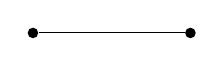
\begin{tikzpicture}[baseline=(current bounding box.center), x=1cm, y=1cm]
\node[gvvertex] (a) at (0,0) {};
\node[gvvertex] (b) at (2,0) {};
\draw[gvedge] (a) -- (b);
\end{tikzpicture}
\\

$2$
&
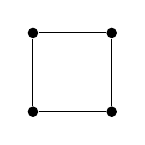
\begin{tikzpicture}[baseline=(current bounding box.center), x=1cm, y=1cm]
\node[gvvertex] (a) at (0,1) {};
\node[gvvertex] (b) at (1,1) {};
\node[gvvertex] (c) at (0,0) {};
\node[gvvertex] (d) at (1,0) {};
\draw[gvedge] (a) -- (b);
\draw[gvedge] (c) -- (d);
\draw[gvedge] (a) -- (c);
\draw[gvedge] (b) -- (d);
\end{tikzpicture}
\\

$3$
&
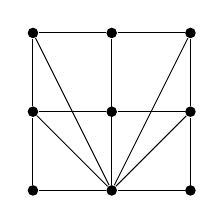
\begin{tikzpicture}[baseline=(current bounding box.center), x=1cm, y=1cm]
\node[gvvertex] (v00) at (0,0) {};
\node[gvvertex] (v10) at (1,0) {};
\node[gvvertex] (v20) at (2,0) {};

\node[gvvertex] (v01) at (0,1) {};
\node[gvvertex] (v11) at (1,1) {};
\node[gvvertex] (v21) at (2,1) {};

\node[gvvertex] (v02) at (0,2) {};
\node[gvvertex] (v12) at (1,2) {};
\node[gvvertex] (v22) at (2,2) {};

\draw[gvedge] (v00) -- (v10) -- (v20);
\draw[gvedge] (v01) -- (v11) -- (v21);
\draw[gvedge] (v02) -- (v12) -- (v22);

\draw[gvedge] (v00) -- (v01) -- (v02);
\draw[gvedge] (v10) -- (v11) -- (v12);
\draw[gvedge] (v20) -- (v21) -- (v22);

\draw[gvedge] (v10) -- (v01);
\draw[gvedge] (v10) -- (v21);
\draw[gvedge] (v10) -- (v02);
\draw[gvedge] (v10) -- (v12);
\draw[gvedge] (v10) -- (v22);
\end{tikzpicture}
\\

$4$
&
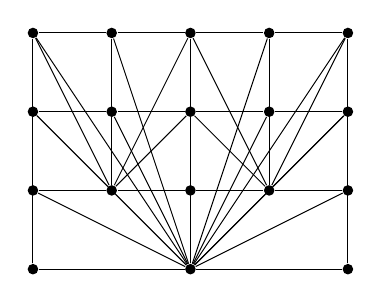
\begin{tikzpicture}[baseline=(current bounding box.center), x=1cm, y=1cm]
\node[gvvertex] (v0m1) at (0,-1) {};
\node[gvvertex] (v2m1) at (2,-1) {};
\node[gvvertex] (v4m1) at (4,-1) {};

\node[gvvertex] (v00) at (0,0) {};
\node[gvvertex] (v10) at (1,0) {};
\node[gvvertex] (v20) at (2,0) {};
\node[gvvertex] (v30) at (3,0) {};
\node[gvvertex] (v40) at (4,0) {};

\node[gvvertex] (v01) at (0,1) {};
\node[gvvertex] (v11) at (1,1) {};
\node[gvvertex] (v21) at (2,1) {};
\node[gvvertex] (v31) at (3,1) {};
\node[gvvertex] (v41) at (4,1) {};

\node[gvvertex] (v02) at (0,2) {};
\node[gvvertex] (v12) at (1,2) {};
\node[gvvertex] (v22) at (2,2) {};
\node[gvvertex] (v32) at (3,2) {};
\node[gvvertex] (v42) at (4,2) {};

\draw[gvedge] (v00) -- (v10) -- (v20) -- (v30) -- (v40);
\draw[gvedge] (v01) -- (v11) -- (v21) -- (v31) -- (v41);
\draw[gvedge] (v02) -- (v12) -- (v22) -- (v32) -- (v42);

\draw[gvedge] (v00) -- (v01) -- (v02);
\draw[gvedge] (v10) -- (v11) -- (v12);
\draw[gvedge] (v20) -- (v21) -- (v22);
\draw[gvedge] (v30) -- (v31) -- (v32);
\draw[gvedge] (v40) -- (v41) -- (v42);

\draw[gvedge] (v0m1) -- (v2m1) -- (v4m1);
\draw[gvedge] (v0m1) -- (v00);
\draw[gvedge] (v4m1) -- (v40);

\draw[gvedge] (v0m1) -- (v01);
\draw[gvedge] (v0m1) -- (v02);

\draw[gvedge] (v4m1) -- (v41);
\draw[gvedge] (v4m1) -- (v42);

\draw[gvedge] (v10) -- (v01);
\draw[gvedge] (v10) -- (v21);
\draw[gvedge] (v10) -- (v02);
\draw[gvedge] (v10) -- (v12);
\draw[gvedge] (v10) -- (v22);

\draw[gvedge] (v30) -- (v21);
\draw[gvedge] (v30) -- (v41);
\draw[gvedge] (v30) -- (v22);
\draw[gvedge] (v30) -- (v32);
\draw[gvedge] (v30) -- (v42);

\draw[gvedge] (v2m1) -- (v0m1);
\draw[gvedge] (v2m1) -- (v4m1);

\draw[gvedge] (v2m1) -- (v00);
\draw[gvedge] (v2m1) -- (v10);
\draw[gvedge] (v2m1) -- (v20);
\draw[gvedge] (v2m1) -- (v30);
\draw[gvedge] (v2m1) -- (v40);

\draw[gvedge] (v2m1) -- (v01);
\draw[gvedge] (v2m1) -- (v11);
\draw[gvedge] (v2m1) -- (v21);
\draw[gvedge] (v2m1) -- (v31);
\draw[gvedge] (v2m1) -- (v41);

\draw[gvedge] (v2m1) -- (v02);
\draw[gvedge] (v2m1) -- (v12);
\draw[gvedge] (v2m1) -- (v22);
\draw[gvedge] (v2m1) -- (v32);
\draw[gvedge] (v2m1) -- (v42);
\end{tikzpicture}
\\

$5$
&
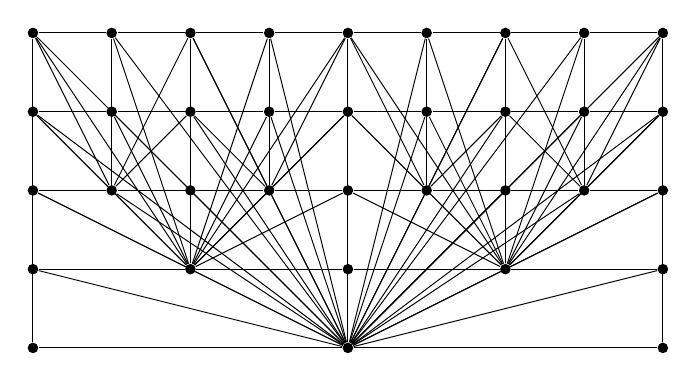
\begin{tikzpicture}[baseline=(current bounding box.center), x=1cm, y=1cm]
\node[gvvertex] (v0m2) at (0,-2) {};
\node[gvvertex] (v4m2) at (4,-2) {};
\node[gvvertex] (v8m2) at (8,-2) {};

\node[gvvertex] (v0m1) at (0,-1) {};
\node[gvvertex] (v2m1) at (2,-1) {};
\node[gvvertex] (v4m1) at (4,-1) {};
\node[gvvertex] (v6m1) at (6,-1) {};
\node[gvvertex] (v8m1) at (8,-1) {};

\node[gvvertex] (v00) at (0,0) {};
\node[gvvertex] (v10) at (1,0) {};
\node[gvvertex] (v20) at (2,0) {};
\node[gvvertex] (v30) at (3,0) {};
\node[gvvertex] (v40) at (4,0) {};
\node[gvvertex] (v50) at (5,0) {};
\node[gvvertex] (v60) at (6,0) {};
\node[gvvertex] (v70) at (7,0) {};
\node[gvvertex] (v80) at (8,0) {};

\node[gvvertex] (v01) at (0,1) {};
\node[gvvertex] (v11) at (1,1) {};
\node[gvvertex] (v21) at (2,1) {};
\node[gvvertex] (v31) at (3,1) {};
\node[gvvertex] (v41) at (4,1) {};
\node[gvvertex] (v51) at (5,1) {};
\node[gvvertex] (v61) at (6,1) {};
\node[gvvertex] (v71) at (7,1) {};
\node[gvvertex] (v81) at (8,1) {};

\node[gvvertex] (v02) at (0,2) {};
\node[gvvertex] (v12) at (1,2) {};
\node[gvvertex] (v22) at (2,2) {};
\node[gvvertex] (v32) at (3,2) {};
\node[gvvertex] (v42) at (4,2) {};
\node[gvvertex] (v52) at (5,2) {};
\node[gvvertex] (v62) at (6,2) {};
\node[gvvertex] (v72) at (7,2) {};
\node[gvvertex] (v82) at (8,2) {};

\draw[gvedge] (v00) -- (v10) -- (v20) -- (v30) -- (v40) -- (v50) -- (v60) -- (v70) -- (v80);
\draw[gvedge] (v01) -- (v11) -- (v21) -- (v31) -- (v41) -- (v51) -- (v61) -- (v71) -- (v81);
\draw[gvedge] (v02) -- (v12) -- (v22) -- (v32) -- (v42) -- (v52) -- (v62) -- (v72) -- (v82);

\draw[gvedge] (v00) -- (v01) -- (v02);
\draw[gvedge] (v10) -- (v11) -- (v12);
\draw[gvedge] (v20) -- (v21) -- (v22);
\draw[gvedge] (v30) -- (v31) -- (v32);
\draw[gvedge] (v40) -- (v41) -- (v42);
\draw[gvedge] (v50) -- (v51) -- (v52);
\draw[gvedge] (v60) -- (v61) -- (v62);
\draw[gvedge] (v70) -- (v71) -- (v72);
\draw[gvedge] (v80) -- (v81) -- (v82);

\draw[gvedge] (v0m1) -- (v2m1) -- (v4m1) -- (v6m1) -- (v8m1);
\draw[gvedge] (v0m2) -- (v4m2) -- (v8m2);

\draw[gvedge] (v0m2) -- (v0m1);
\draw[gvedge] (v4m2) -- (v4m1);
\draw[gvedge] (v8m2) -- (v8m1);

\draw[gvedge] (v0m1) -- (v00);
\draw[gvedge] (v2m1) -- (v20);
\draw[gvedge] (v4m1) -- (v40);
\draw[gvedge] (v6m1) -- (v60);
\draw[gvedge] (v8m1) -- (v80);

\draw[gvedge] (v0m2) -- (v4m2);
\draw[gvedge] (v4m2) -- (v8m2);

\draw[gvedge] (v0m2) -- (v00);
\draw[gvedge] (v0m2) -- (v01);
\draw[gvedge] (v0m2) -- (v02);

\draw[gvedge] (v8m2) -- (v80);
\draw[gvedge] (v8m2) -- (v81);
\draw[gvedge] (v8m2) -- (v82);

\draw[gvedge] (v10) -- (v01);
\draw[gvedge] (v10) -- (v21);
\draw[gvedge] (v10) -- (v02);
\draw[gvedge] (v10) -- (v12);
\draw[gvedge] (v10) -- (v22);

\draw[gvedge] (v30) -- (v21);
\draw[gvedge] (v30) -- (v41);
\draw[gvedge] (v30) -- (v22);
\draw[gvedge] (v30) -- (v32);
\draw[gvedge] (v30) -- (v42);

\draw[gvedge] (v50) -- (v41);
\draw[gvedge] (v50) -- (v61);
\draw[gvedge] (v50) -- (v42);
\draw[gvedge] (v50) -- (v52);
\draw[gvedge] (v50) -- (v62);

\draw[gvedge] (v70) -- (v61);
\draw[gvedge] (v70) -- (v81);
\draw[gvedge] (v70) -- (v62);
\draw[gvedge] (v70) -- (v72);
\draw[gvedge] (v70) -- (v82);

\draw[gvedge] (v2m1) -- (v0m1);
\draw[gvedge] (v2m1) -- (v4m1);
\draw[gvedge] (v2m1) -- (v00);
\draw[gvedge] (v2m1) -- (v10);
\draw[gvedge] (v2m1) -- (v20);
\draw[gvedge] (v2m1) -- (v30);
\draw[gvedge] (v2m1) -- (v40);
\draw[gvedge] (v2m1) -- (v01);
\draw[gvedge] (v2m1) -- (v11);
\draw[gvedge] (v2m1) -- (v21);
\draw[gvedge] (v2m1) -- (v31);
\draw[gvedge] (v2m1) -- (v41);
\draw[gvedge] (v2m1) -- (v02);
\draw[gvedge] (v2m1) -- (v12);
\draw[gvedge] (v2m1) -- (v22);
\draw[gvedge] (v2m1) -- (v32);
\draw[gvedge] (v2m1) -- (v42);

\draw[gvedge] (v6m1) -- (v4m1);
\draw[gvedge] (v6m1) -- (v8m1);
\draw[gvedge] (v6m1) -- (v40);
\draw[gvedge] (v6m1) -- (v50);
\draw[gvedge] (v6m1) -- (v60);
\draw[gvedge] (v6m1) -- (v70);
\draw[gvedge] (v6m1) -- (v80);
\draw[gvedge] (v6m1) -- (v41);
\draw[gvedge] (v6m1) -- (v51);
\draw[gvedge] (v6m1) -- (v61);
\draw[gvedge] (v6m1) -- (v71);
\draw[gvedge] (v6m1) -- (v81);
\draw[gvedge] (v6m1) -- (v42);
\draw[gvedge] (v6m1) -- (v52);
\draw[gvedge] (v6m1) -- (v62);
\draw[gvedge] (v6m1) -- (v72);
\draw[gvedge] (v6m1) -- (v82);

\draw[gvedge] (v4m2) -- (v0m1);
\draw[gvedge] (v4m2) -- (v2m1);
\draw[gvedge] (v4m2) -- (v4m1);
\draw[gvedge] (v4m2) -- (v6m1);
\draw[gvedge] (v4m2) -- (v8m1);

\draw[gvedge] (v4m2) -- (v00);
\draw[gvedge] (v4m2) -- (v10);
\draw[gvedge] (v4m2) -- (v20);
\draw[gvedge] (v4m2) -- (v30);
\draw[gvedge] (v4m2) -- (v40);
\draw[gvedge] (v4m2) -- (v50);
\draw[gvedge] (v4m2) -- (v60);
\draw[gvedge] (v4m2) -- (v70);
\draw[gvedge] (v4m2) -- (v80);

\draw[gvedge] (v4m2) -- (v01);
\draw[gvedge] (v4m2) -- (v11);
\draw[gvedge] (v4m2) -- (v21);
\draw[gvedge] (v4m2) -- (v31);
\draw[gvedge] (v4m2) -- (v41);
\draw[gvedge] (v4m2) -- (v51);
\draw[gvedge] (v4m2) -- (v61);
\draw[gvedge] (v4m2) -- (v71);
\draw[gvedge] (v4m2) -- (v81);

\draw[gvedge] (v4m2) -- (v02);
\draw[gvedge] (v4m2) -- (v12);
\draw[gvedge] (v4m2) -- (v22);
\draw[gvedge] (v4m2) -- (v32);
\draw[gvedge] (v4m2) -- (v42);
\draw[gvedge] (v4m2) -- (v52);
\draw[gvedge] (v4m2) -- (v62);
\draw[gvedge] (v4m2) -- (v72);
\draw[gvedge] (v4m2) -- (v82);
\end{tikzpicture}
% \\

% \hline
\end{tabular}
\caption{Grid views of the first five middle-all-connected iterative gadgets \(\Lambda_k^{\mathrm{mid}}\).}
\label{fig:middle-all-connected-grid-views}
\end{figure}